%% \chapter[htoc-titlei][hhead-titlei]{htitlei}
%% -----------------------------------------------------------------------------
\chapter[Monte Carlo simulation][Monte Carlo simulation]{Monte Carlo simulation}
\label{ch:mc}

{\color{red}
  I learned a lot about these generators (at least MadGraph+pythia),
  so I thought it would be fun to write a bit about them here.
  This chapter may get dropped if I run out of time.
}

%% -----------------------------------------------------------------------------
\section{Event Generation}

{\color{red} What is an event. Brief overview of the different pieces that need
  to be calculated before going into detail}

  \begin{figure}[p]
    \centering
    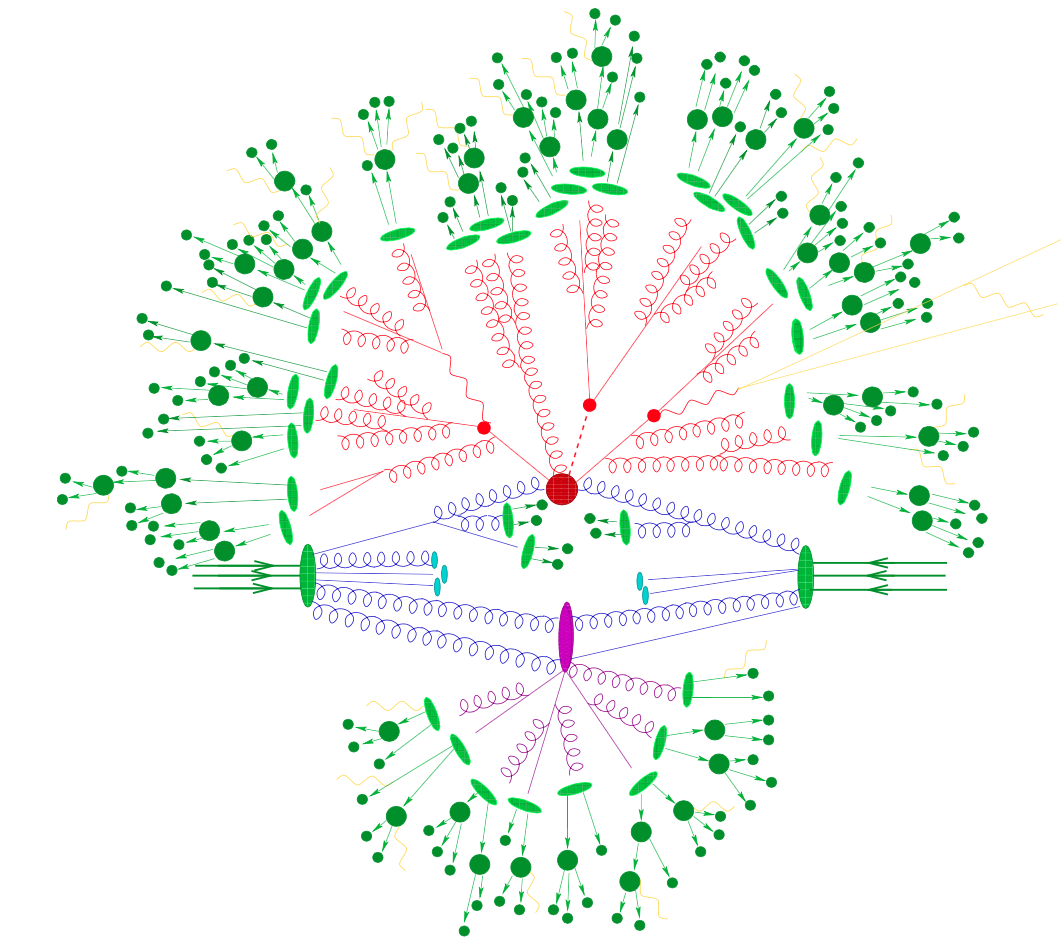
\includegraphics[width=\textwidth, clip=true, trim=0 0 0 0]
    {figs/mc_gen/full_mc_event.png}
    \caption[
      Pictorial representation of a $t\bar{t}H$ event as produced by an event
      generator~\cite{Gleisberg:2008ta}.
    ]{
      Pictorial representation of a $t\bar{t}H$ event as produced by an event
      generator.
      The hard interaction (big red blob) is followed by the decay of both top
      quarks and the Higgs boson (small red blobs).
      Additional hard QCD radiation is produced (red) and a secondary
      interaction takes place (purple blob) before the final-state partons
      hadronize (light green blobs) and hadrons decay (dark green blobs).
      Photon radiation occurs at any stage (yellow)~\cite{Gleisberg:2008ta}.
    }
    \label{fig:mc_event}
\end{figure}


%% - - - - - - - - - - - - - - - - - - - - - - - - - - - - - - - - - - - - - - -
\subsection{Underlying event}

%% - - - - - - - - - - - - - - - - - - - - - - - - - - - - - - - - - - - - - - -
\subsection{Matrix element}

%% - - - - - - - - - - - - - - - - - - - - - - - - - - - - - - - - - - - - - - -
\subsection{Parton shower}

%% - - - - - - - - - - - - - - - - - - - - - - - - - - - - - - - - - - - - - - -
\subsection{Jet matching}
\label{sec:jet_matching}

{\color{red} Talk about matching. Probably use several figures to help explain
  this topic. Probably also talk about these DJR plots, and how we want them
  to look}

{\color{red} Add info about HFOR here}

%% -----------------------------------------------------------------------------
\section{Detector simulation}

{\color{red} Probably something brief about how detector simulation is done, and
  the difference between full/fast sim}

